%% LyX 2.1.4 created this file.  For more info, see http://www.lyx.org/.
%% Do not edit unless you really know what you are doing.
\documentclass[twocolumn,english]{article}
\usepackage[latin9]{inputenc}
\usepackage[landscape]{geometry}
\geometry{verbose,tmargin=0.5in,bmargin=0.75in,lmargin=0.5in,rmargin=0.5in}
\usepackage{float}
\usepackage{booktabs}
\usepackage{graphicx}

\makeatletter

%%%%%%%%%%%%%%%%%%%%%%%%%%%%%% LyX specific LaTeX commands.
%% Because html converters don't know tabularnewline
\providecommand{\tabularnewline}{\\}

%%%%%%%%%%%%%%%%%%%%%%%%%%%%%% User specified LaTeX commands.





\providecommand{\tabularnewline}{\\}

\setlength{\columnsep}{0.25in}
\usepackage{xcolor}
\usepackage{textcomp}
\usepackage{listings}
\lstset{
  language=SQL,
  tabsize=2,
  frame=single,
  basicstyle=\small\ttfamily,
  keepspaces=true,
  moredelim=[is][\underbar]{*}{*},
}



\usepackage{babel}
\usepackage{listings}
\renewcommand{\lstlistingname}{Listing}

\makeatother

\usepackage{babel}
\usepackage{listings}
\renewcommand{\lstlistingname}{Listing}

\begin{document}

\title{Reference Sheet for CO130 Databases}


\date{Spring 2017}

\maketitle

\section{Benefits of Databases}
\begin{enumerate}
\item Organised and efficient. 
\item Minimise data duplication. 
\item Support concurrent actions. 
\item Support multiple users, controls who can access which data. 
\item Support recovery from failures. 
\end{enumerate}

\subsection{Transactions}
\begin{enumerate}
\item \emph{Atomicity}: if one part fails, whole transaction fails (rolls
back). 
\item \emph{Consistency}: must not leave database in inconsistent state. 
\item \emph{Isolation}: executed as if no other transaction is occurring
(serialised execution).
\item \emph{Durability}: Results of successful transactions not lost. 
\end{enumerate}

\section{Relational Model}
\begin{enumerate}
\item \emph{Database}: one or more relations. 
\item \emph{Database schema}: schemas for all relations. 
\item \emph{Relation}: heading and body: set of tuples of the form $\left(A_{1}:S_{1}=V_{1},\dots,A_{n}:S_{n}=V_{n}\right)$. 
\item \emph{Relation schema}: name of relation and heading. 
\item \emph{Heading}: unordered set of attributes (names and types). 
\item \emph{Body}: unnordered set of tuples (sets of attribute values). 
\end{enumerate}

\subsection{Entity-Relationship Digrams}
\begin{enumerate}
\item \emph{Entity sets} (rectangles): distinguishable entities tht share
same properties. 
\item \emph{Relationship} (diamonds): captures how two or more entity sets
are related. 
\item \emph{Attributes} (circles): property of entity, primary key attributes
underlined. 
\end{enumerate}

\subsubsection{Complex Attributes}
\begin{enumerate}
\item \emph{Composite} (tree): subdivided e.g. address into road, city,
postcode. 
\item \emph{Multivalued} (double border): set of values e.g. several phones. 
\item \emph{Derived} (dotted line and border): computed from other values
e.g. age from DoB. 
\end{enumerate}

\subsubsection{Cardinality Constraints and Entity Set Participation}
\begin{enumerate}
\item \emph{One-to-one}, \emph{one-to-many}, \emph{many-to-many}: add labels
1 1, 1 N, and M N to relationship respectively. 
\item \emph{Total participation}: use double line, requires all entities
to participate in a relationship. 
\item \emph{Participation bounds}: use .. notation in labels. 
\end{enumerate}

\subsubsection{Fan Traps and Chasm Traps}

\emph{Fan traps}: ambiguous paths exist between entities. Can be solved
by changing structure (e.g. staff - dept - faculty).

\begin{center}
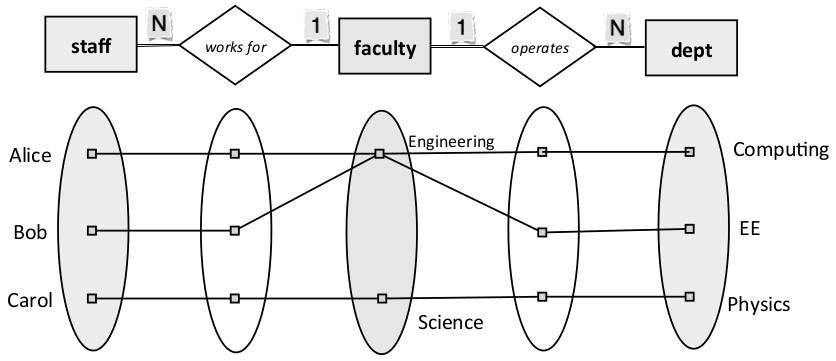
\includegraphics[scale=0.2]{img/fan}
\par\end{center}

\noindent \emph{Chasm traps}: suggests a relationship between entities
but one doesn't exist. Can be solved by adding a new relationship
(e.g. between dept and PC).

\begin{center}
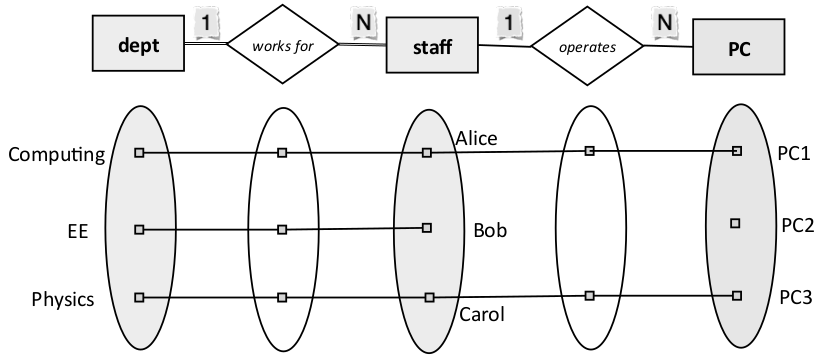
\includegraphics[scale=0.2]{img/chasm}
\par\end{center}


\subsubsection{More relationships}
\begin{enumerate}
\item \emph{Multiway relationships}: can have relationships between more
than two entity sets. 
\item \emph{Roles}: one entity set can have more than one role (e.g. prequel
and sequel), draw multiple lines and label. 
\item \emph{is-a relationships}: hollow arrow head, can form hierarchies. 
\end{enumerate}

\subsubsection{More Entities}

\emph{Weak entities} (double rectangle, double diamond): cannot be
uniquely identified on own attributes and requires a strong entity
to exist. Identified using primary key of strong entity and one ore
more attributes of itself (dotted underlined). E.g. room cannot exist
without building that contains it.


\subsection{Relation Schemas from ER Models}


\subsubsection{Joins and Keys}
\begin{enumerate}
\item Primary key: uniquely identifies tuple 
\item Foreign key: primary key used in different table 
\end{enumerate}

\subsubsection{Entity Sets and attributes}

Mapped directly to realtion with the same attributes. E.g.

\begin{lstlisting}
actor(*ID*, firstname, lastname, housno, roadname, city)
actor_cars(*actorID*, *carID*)

create table actor (
	ID           int,
	firstname    varchar(30),
	lastname     varchar(30),
	houseno      int,
	roadname     varchar(30),
	city         varchar(40),

	primary key (ID)
)

create table actor_cars (
	actorID      int,
	carID        varchar(10),
	
	primary key (actorID, carID),
	foreign key (actorID) references actor.ID
)
\end{lstlisting}

\begin{enumerate}
\item \emph{Composite attributes}: flatten to contain only simple attributes. 
\item \emph{Multivalued attributes}: own relation mapped back to entity
set using foreign key. 
\item \emph{Derived attributes}: not supported by relational model. 
\end{enumerate}

\paragraph{Weak Entity Sets}

Mapped to its own relation and attributes but includes primary key
of strong attribute with on delete cascade constraint.


\subsubsection{Relationships}

\emph{Many-to-many}: new relation with two foreign keys. E.g.

\begin{lstlisting}
person(*ID*, otherattributes)
car(*regno*, otherattributes)
drive(*personID*, *regno*, otherattributes)

create table drive (
	personID    varchar(10),
	regno       varchar(12),

	primary key (personID, regno),
	foreign key (personID) references person.ID on delete.cascade,
	foreign key (regno) references car.regno on delete.cascade
)
\end{lstlisting}


\noindent \emph{One-to-many} and \emph{one-to-one}: directly include
primary key of the One relation as foreign key in the Many relation.
E.g.

\begin{lstlisting}
person(*ID*, otherattributes)
car(*regno*, personID, otherattributes)

create table car (
	regno       varchar(12),
	personID    varchar(10),

	primary key (regno),
	foreign key (personID) references person.ID
)
\end{lstlisting}



\paragraph{Multiway Relationships}

Include primary keys from all entity sets of foreign keys. Primary
key is formed by foreign keys of the many entity sets.


\paragraph{Roles in Relationships}

Each role is mapped to a foreign key attribute.


\paragraph{is-a Relationships}

Include primary key of root level entity set with every lower-level
entity set


\subsubsection{Database Design Maxims}
\begin{enumerate}
\item Model the `real world' as much as possible 
\item Keep it as simple as possible 
\item Express each property once only 
\end{enumerate}

\section{Relational Algebra}
\begin{enumerate}
\item \emph{Union} $R\cup S$: set of tuples in $R$ or $S$. 
\item \emph{Difference} $R-S$: set of tuples in $R$ but not $S$. 
\item \emph{Intersection} $R\cap S$: set of tuples in $R$ and $S$. 
\item \emph{Projection} $\pi_{A}(R)$: relation $R$ with attributes $A$
only. 
\item \emph{Condition} $\sigma_{p}(R)$: all tuples of $R$ that satisfy
the condition $p$. 
\item \emph{Cartesian product} $R\times S$: all tuples that can be paired
by including a tuple from $R$ and a tuple from $S$. 
\item \emph{Natural join} $R\bowtie S$: all tuples that can be `joined'
using all matching attributes of $R$ and $S$. 
\item \emph{Left outer}, \emph{right outer}, \emph{full outer join}: keep
entries from left, right, both set(s) which do not match attributes
in the other. 
\item \emph{Renaming} $\rho_{n_{1}/o_{1},\dots,n_{n},o_{n}}(R)$: changes
name of attribute $o_{1}$ to $n_{1}$, ..., $o_{n}$ to $n_{n}$. 
\end{enumerate}

\paragraph{Relational Expressions}

Used for \emph{retrieval}, \emph{updates} (insert, change, delete
data), defining \emph{constraints}, \emph{derived relations} (define
one relation in terms of others), \emph{concurrency} (defining data
to use for concurrent actions), \emph{access control} (define data
over which permissions should be granted).


\section{Functional Dependencies}
\begin{enumerate}
\item \emph{Functional Dependency}: constraint that if two tuples of a relation
$R$ agree on attributes $A_{1},A_{2},\dots,A_{n}$ they also agree
on $B_{1},B_{2},\dots,B_{m}$: $A_{1},A_{2},\dots,A_{n}\rightarrow B_{1},B_{2},\dots,B_{m}$. 
\item \emph{Superkey}: a set of attributes that functionally determines
all the other attributes of the relation. 
\item \emph{Candidate Key}: if there is no proper subset of the superkey. 
\end{enumerate}

\paragraph{Splitting and Combining Dependencies}
\begin{enumerate}
\item \emph{Splitting Rule}: if $A,B,C,D,E\rightarrow X,Y,Z$ then $A,B,C,D,E\rightarrow X$,
$A,B,C,D,E\rightarrow Y$ and $A,B,C,D,E\rightarrow Z$. 
\item \emph{Combining Rule}: if $A,B,C,D,E\rightarrow X$, $A,B,C,D,E\rightarrow Y$
and $A,B,C,D,E\rightarrow Z$ then $A,B,C,D,E\rightarrow X,Y,Z$. 
\end{enumerate}

\paragraph{Trivial Dependencies}
\begin{enumerate}
\item \emph{Trivial Dependency Rule}: if $A,B,C,D,E\rightarrow A,B,X,Y,Z$
then $A,B,C,D,E\rightarrow X,Y,Z$ and vice versa. 
\item \emph{Trivial FD}: all attributes on the RHS are also on the LHS. 
\end{enumerate}

\paragraph{Closure of Attribute Sets}
\begin{enumerate}
\item Consider a set of attributes $L$. Its \emph{closure under} $F$,
$L^{+}$ is the set of all attributes functionally determined by $L$. 
\item $L$ is a superkey of $R$ if $L^{+}$ contains all the attributes
of $R$. 
\item If $\mbox{RHS}\subseteq\mbox{LHS}^{+}$, then $\mbox{LHS}\rightarrow\mbox{RHS}$. 
\end{enumerate}

\paragraph{Armstrong's Axioms}

Sound and complete axiomatisation of FDs. 
\begin{enumerate}
\item \emph{Reflexivity}: $\alpha\rightarrow\beta$ always holds if $\beta\subseteq\alpha$ 
\item \emph{Augmentation}: if $\alpha\rightarrow\beta$ then $\alpha\gamma\rightarrow\beta\gamma$
(note that $\alpha\gamma=\gamma\alpha$). 
\item \emph{Transivitiy}: if $\alpha\rightarrow\beta$ and $\beta\rightarrow\gamma$
then $\alpha\rightarrow\gamma$. 
\end{enumerate}

\paragraph{Additional Rules}

Can be derived from the axioms. 
\begin{enumerate}
\item \emph{Union}: if $\alpha\rightarrow\beta$ and $\alpha\rightarrow\gamma$
then $\alpha\rightarrow\beta\gamma$. 
\item \emph{Decomposition}: if $\alpha\rightarrow\beta\gamma$ then $\alpha\rightarrow\beta$
and $\alpha\rightarrow\gamma$. 
\item \emph{Pseudotransitivity}: if $\alpha\rightarrow\beta$ and $\delta\beta\rightarrow\gamma$
then $\delta\alpha\rightarrow\gamma$. 
\end{enumerate}

\paragraph{Finding Closure of Functional Dependency Set}

Start with $F^{+}=F$. Repeat (until $F^{+}$ doesn't change): 
\begin{enumerate}
\item Apply reflexivity and augmentation. Add new FDs to $F^{+}$. 
\item Apply transivity to FDs in $F^{+}$and add new FD to $F^{+}$. 
\end{enumerate}

\paragraph{Covers of Functional Dependency Sets}
\begin{enumerate}
\item $F_{1}$ and $F_{2}$ are equivalent if each implies the other. They
are \emph{covers} of each other. 
\item A cover is \emph{canonical} if:

\begin{enumerate}
\item Each LHS is unique. 
\item We cannot delete any FD from the cover and have an equivalent FD set. 
\item We cannot delete any attribute from any FD and still have an equivalent
FD set. 
\end{enumerate}
\end{enumerate}

\paragraph{Computing a Canonical Cover}

Repeat over $F$ (until it doesn't change): 
\begin{enumerate}
\item Union rule for all possible dependencies (if $\alpha\rightarrow\beta$
and $\alpha\rightarrow\gamma$ then $\alpha\rightarrow\beta\gamma$). 
\item Remove any extraneous attributes (often easiest by inspection).

\begin{enumerate}
\item LHS $X$ is extraneous if $\mbox{RHS}\subseteq\left\{ \mbox{LHS}-X\right\} ^{+}$
under the FD set. 
\item RHS $X$ is extraneous if $X\in\mbox{LHS}^{+}$ under the FD set with
$X$ removed from its FD RHS. 
\end{enumerate}
\end{enumerate}

\section{Normalisation}


\subsection{Decomposition}
\begin{enumerate}
\item \emph{Decomposition}: Given $R$, decompose it into $S$ and $T$
such that $\mbox{attr}\left(R\right)=\mbox{attr}\left(S\right)\cup\mbox{attr}\left(T\right)$,
$S=\pi_{\mbox{attr}\left(S\right)}\left(R\right)$, $T=\pi_{\mbox{attr}\left(T\right)}\left(R\right)$. 
\item \emph{Lossless Decomposition}: At least one of the following FDs holds:

\begin{enumerate}
\item $\mbox{attr}\left(S\right)\cap\mbox{attr}\left(T\right)\rightarrow\mbox{attr}\left(S\right)$ 
\item $\mbox{attr}\left(S\right)\cap\mbox{attr}\left(T\right)\rightarrow\mbox{attr}\left(T\right)$ 
\end{enumerate}
\item \emph{Dependency Preserving Decompositon}: We can check the functional
dependencies of $R$ without joining $S$ and $T$. 
\end{enumerate}

\subsection{Boyce-Codd Normal Form}

A relation is in \emph{BCNF} iff for all non-trivial FDs, the LHS
of every FD is a superkey (contains a key).


\paragraph{Decomposition into BCNF}

For a relation $R$. While there are relations $V$ with violating
FDs: 
\begin{enumerate}
\item Find a non-trivial FD $\mbox{LHS}\rightarrow\mbox{RHS}$ s.t.:

\begin{enumerate}
\item LHS is not a superkey of $R$ 
\item $\mbox{LHS}\cap\mbox{RHS}=\{\}$ 
\end{enumerate}
\item Remove $V$ from the current decompositions 
\item Add relation $\left(\mbox{LHS}\cup\mbox{RHS}\right)$ to decompositions. 
\item Add relation $\left(\mbox{attr}\left(V\right)-\mbox{RHS}\right)$
to decompositions. 
\end{enumerate}
Note that BCNF is lossless but not necessarily dependency preserving.
It eliminates redundancy.


\subsection{Third Normal Form}

A relation is in \emph{3NF} iff for all non-trivial FDs, the LHS of
every FD is a superkey or if every attribute on the RHS of a FD is
prime (a member of any key of the relation).


\paragraph{Decomposition into 3NF}

$C$ is a canonical cover (minimal FD set) for $R$. Then start with
the set $D=\{\}$ of decomposed relations. 
\begin{enumerate}
\item For each FD $\mbox{LHS}\rightarrow\mbox{RHS}$ in $C$, add a new
relation $\left(\mbox{LHS}\cup\mbox{RHS}\right)$ to the set of decomposed
relations $D$. 
\item For each relation $R$ in $D$ that is a subset of another relation
in $D$, remove $R$ from $D$. 
\item If none of the relations in $D$ includes a key for $R$, add a new
relation(key) to $D$. 
\end{enumerate}
3NF is lossless and dependency preserving but does not necessarily
eliminate redundancy.


\section{Structured Query Language}


\subsection{Relational Algebra to SQL}

\noindent 
\begin{table}[H]
\noindent \centering{}%
\begin{tabular}{cc}
\toprule 
\addlinespace
\emph{Relation Algebra}  & \emph{SQL}\tabularnewline
\midrule
\addlinespace
$R\cup S$  & \texttt{R }\texttt{\textbf{union}}\texttt{ S}\tabularnewline
\addlinespace
$R\cap S$  & \texttt{R }\texttt{\textbf{intersect}}\texttt{ S}\tabularnewline
\addlinespace
$R-S$  & \texttt{R }\texttt{\textbf{except}}\texttt{ S}\tabularnewline
\addlinespace
$\pi_{\mbox{attributes}}\left(R\right)$  & \texttt{\textbf{select}}\texttt{ attributes }\texttt{\textbf{from}}\texttt{
R}\tabularnewline
\addlinespace
$\sigma_{\mbox{condition}}\left(R\right)$  & \texttt{\textbf{from}}\texttt{ R }\texttt{\textbf{where}}\texttt{
condition}\tabularnewline
\addlinespace
$R\times S$  & \texttt{R,S or R }\texttt{\textbf{cross join}}\texttt{ S}\tabularnewline
\addlinespace
$R\bowtie S$  & \texttt{R }\texttt{\textbf{natural join}}\texttt{ S}\tabularnewline
\addlinespace
$R\bowtie_{\mbox{condition}}S$  & \texttt{R }\texttt{\textbf{join}}\texttt{ S }\texttt{\textbf{on}}\texttt{
condition}\tabularnewline
\midrule
\addlinespace
Relation  & \texttt{\textbf{Table}}\tabularnewline
\addlinespace
Relational Expression  & \texttt{\textbf{Views}}\tabularnewline
\addlinespace
Tuple  & \texttt{Row}\tabularnewline
\addlinespace
Attribute  & \texttt{Column}\tabularnewline
\addlinespace
Domain  & \texttt{Type}\tabularnewline
\bottomrule
\end{tabular}
\end{table}



\subsection{Some Common Types}
\begin{enumerate}
\item \texttt{int, smallint, real, double precision, float(n), numeric(p,d),
decimal(p,d)} - usual arithmetic operators are available. 
\item \texttt{char, char(n), varchar(n), clob/tect, ...} - operators include
\texttt{\textbar{}\textbar{}} (concatenation), \texttt{like} (performs
pattern matching: \texttt{\_} for any char, \texttt{\%} for zero or
more chars), \texttt{similar to} (for regex matches). 
\item \texttt{bit(n), byte(n), blob}. 
\item \texttt{boolean} - based on three-valued logic (can be \texttt{unknown})
- operators include \texttt{between}, \texttt{not between}, \texttt{in},
\texttt{not in}. 
\item \texttt{date, time, timestamp}. 
\item \texttt{...} 
\end{enumerate}

\subsection{Null}

Attribute value used to represent values that are missing, not applicable,
or witheld. 
\begin{enumerate}
\item Any arithmetic involving \texttt{null} results in \texttt{null}. 
\item Comparisons with \texttt{null} give \texttt{unknown}. 
\item \texttt{null} will never match another value, need to use \texttt{is
null} or \texttt{is not null}. 
\end{enumerate}

\subsection{Queries}
\begin{enumerate}
\item \texttt{select atts from table where conds} used to query datbase. 
\item \texttt{{*}} used to select all attributes. 
\item \texttt{as newName} used to rename attributes. 
\item \texttt{order by att} used to sort results by a column. 
\item \texttt{table inner join} \texttt{table}, \texttt{left outer join},
\texttt{right outer join}, \texttt{full outer join}. 
\item \texttt{on cond} to join given a predicate. 
\item \texttt{using att} to join on a specific attribute. 
\item \texttt{distinct} to eliminate duplicates. 
\item \texttt{sum}, \texttt{avg}, \texttt{min}, \texttt{max}, \texttt{count}
as aggregate functions. 
\item \texttt{group by} ... \texttt{having} used to group tuples in resulting
relation. Note any non-aggregates used in the \texttt{having} filter
must be included in the \texttt{group by} list.
\item \texttt{some} (any) and \texttt{all} to compare a value against some
or all values returned by a subquery. 
\item \texttt{exists} and \texttt{not exists} to test whether a relation
is empty or not 
\item \texttt{unique} or \texttt{not unique} to test if a relation has duplicates.
\end{enumerate}

\subsubsection{Subqueries}
\begin{enumerate}
\item \emph{Scalar subquery} produces single value. Typically a \texttt{select}
with an aggregate function.
\item \emph{Set subquery} produces set of distinct values (column). Typically
used for membership (\texttt{in} or \texttt{not in}) or comparisons
(\texttt{some} or \texttt{all}).
\item \emph{Relation subquery} produces relation. Typically used as operand
of products, \texttt{join}s, \texttt{union}s, \texttt{intersect}s,
\texttt{except}s, \texttt{exists}, \texttt{not exists}, \texttt{unique}
or \texttt{not unique}.
\end{enumerate}

\subsubsection{Advanced Queries}
\begin{enumerate}
\item \texttt{limit n} to specify number of records to return.
\item \texttt{like ...} used to search for specified pattern, \texttt{\_}
matches exactly one character, \texttt{\%} matches zero or more characters.
\end{enumerate}

\subsection{Data Definition}
\begin{enumerate}
\item \texttt{create table name (atts)} to create a relation.
\item \texttt{drop table table} to delete a relation.
\item \texttt{alter table table}, then \texttt{add (atts)} or \texttt{drop
(atts)}.
\end{enumerate}

\paragraph{Constraints}
\begin{enumerate}
\item \texttt{not null} prohibits assignment of \texttt{null}s.
\item \texttt{default} sets default value for attribute.
\item \texttt{auto\_increment (start, by)} allows a unique number to be
generated by default.
\item \texttt{primary key (atts)} (must be unique, \texttt{null}s not permitted).
\item \texttt{foreign key (atts) references table (atts)} checks that attributes
in relation match value of a candidate key in a referenced relation
(\emph{referential integrity}).
\item \texttt{unique (atts)} to ensure no two tuples have same set of values
for listed attributes.
\item \texttt{check (expr)} can check an arbitrary expression involving
several attributes and/or a query.
\item Constraints should be named using \texttt{constraint constraintName
...}.
\item \texttt{on update cascade}, \texttt{on delete cascade} maintains referential
integrity by cascading updates / deletions to the foreign key.
\item \texttt{on update set default}, \texttt{on delete set null} another
option that will lead to unmatched tuples.
\end{enumerate}

\subsubsection{Views}

Relations defined using a query, not physically stored. Can be used
to:
\begin{enumerate}
\item Declare commonly used subqueries.
\item Declare a relation over several relations using products, joins.
\item Declare a relation over calculated expressions and aggregated data.
\item Partition data using a selection.
\item Restrict access to a relation by providing access only to a view.
\end{enumerate}
\emph{Materialised views}, stored and kept up to date rather than
being recomputed each time. \emph{Updatable views} usually don't make
sense.


\subsubsection{Indexes}

Copies of an attribute's data that are automatically maintained by
RDBMS but can be searched quickly. Use \texttt{create index name on
table (atts)}.


\subsection{Data Manipulation}
\begin{enumerate}
\item \texttt{insert into table (atts) values (atts), (atts), ...} adds
tuples to a relation. Can use a subquery instead of inserting individual
tuples.
\item \texttt{delete from table where ...} to delete tuple attributes.
\item \texttt{update table set ... where ...} updates tuple attributes.
\item \texttt{case when ... then else end} is often useful in update expressions.
\end{enumerate}

\section{Transactions}
\begin{enumerate}
\item \texttt{start transaction} explicitly starts a transaction.
\item \texttt{commit} and \texttt{rollback} commit and rollback modifications
respectively.
\end{enumerate}
Ensuring ACID:
\begin{enumerate}
\item \emph{Atomicity and Durability}: Rollback possible using a recovery
system. DBMS checks logs. Compensating transactions must be possible.
RAID / replicated disks should be used to guard against disk failure.
\item \emph{Consistency}: Up to the programmer to ensure using constraints.
\item \emph{Isolation}: Use a concurrency control system. E.g. allow concurrent
reads or concurrent read / writes if they are on different relations.
Isolation levels:

\begin{enumerate}
\item \emph{Read uncommitted}: uncommitted data changed by other concurrent
transactions can be read - \emph{dirty reads}.
\item \emph{Read committed}: Only data \emph{committed} by other concurrent
transactions can be read. \emph{Non-repeatable reads} are possible.
\item \emph{Repeatable read}: Guarantees all tuples can be returned by a
query will be included if the query is repeated, but might return
additional newly committed tuples (\emph{phantom reads}).
\item \emph{Serializable}: Guarantees isolution.
\end{enumerate}
\end{enumerate}

\section{Storage and File Structure}


\subsection{Database Servers}
\begin{enumerate}
\item Clients send requests, transactions executed on server, results shipped
back to client.
\item Communicated through a remote procedure call.
\item Open Database Connectivity / JDBC are API standards for sending SQL
requests.
\end{enumerate}
\begin{center}
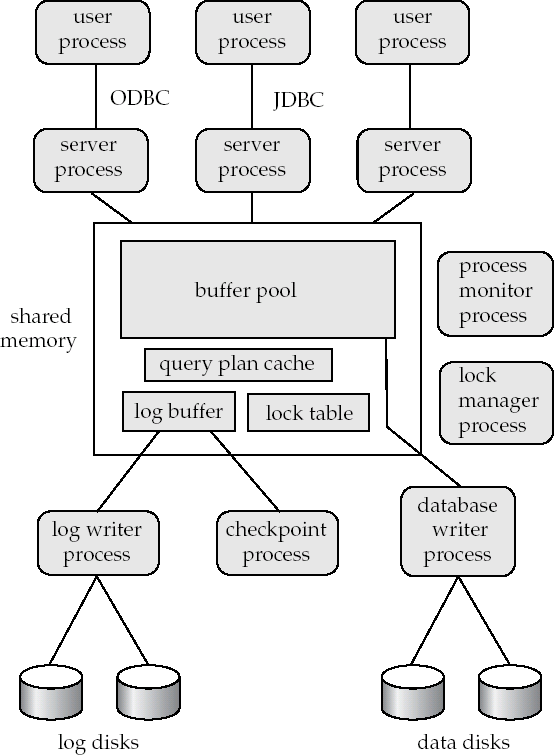
\includegraphics[scale=0.2]{img/database-processes}
\par\end{center}

\noindent All database processes can access shared memory. Systems
implement mutual exclusion using semaphores or atomic instructions.


\subsection{Storage}
\begin{enumerate}
\item \emph{Volatile storage}: loses contents when power switched off.
\item \emph{Non-volatile storage}: contents persist even when power switched
off.
\end{enumerate}

\paragraph{Physical storage media}
\begin{enumerate}
\item \emph{Cache}: fastest and most costly; volatile; managed by system
hardware.
\item \emph{Main memory}: fast; too small or expensive to store a database;
volatile.
\item \emph{Flash memory}: fast reads but slow writes; can only written
to once - but locations can be erased and written to again (limited
number of write/erase cycles, erasing has to be done to entire bank
of memory); non-volatile.

\begin{enumerate}
\item NOR: lower capacity, sometimes used to store program code in embedded
devices.
\item NAND: higher capacity, sometimes used as portable data storage.
\end{enumerate}
\item \emph{Magnetic disk}: uses spinning disk, magnetic reads and writes;
long-term storage of data; data must be moved through main memory;
direct-access (read in any order); survives power-failure and system
crashes (but rare disk failures).
\item \emph{Optical storage} (e.g. CD-ROM, DVD): slow reads and writes;
uses spinning disk and laser; non-volatile; used in jukebox systems.
\item \emph{Tapes}: slow; high capacity; sequential-access; non-volatile;
used for backups and archives - tape jukeboxes can store hundreds
of terabytes. Cheapest storage medium.
\end{enumerate}

\paragraph{Storage Hierarchy}
\begin{enumerate}
\item \emph{Primary storage}: Fastest media but volatile (cache, main memory).
\item \emph{Secondary storage}: Non-volatile, moderately fast, on-line storage
(fash, magnetic disks).
\item \emph{Tertiary storage}: Non-volatile, slow access time (magnetic
tape, optical storage).
\end{enumerate}

\paragraph{Magnetic Disks}

\begin{center}
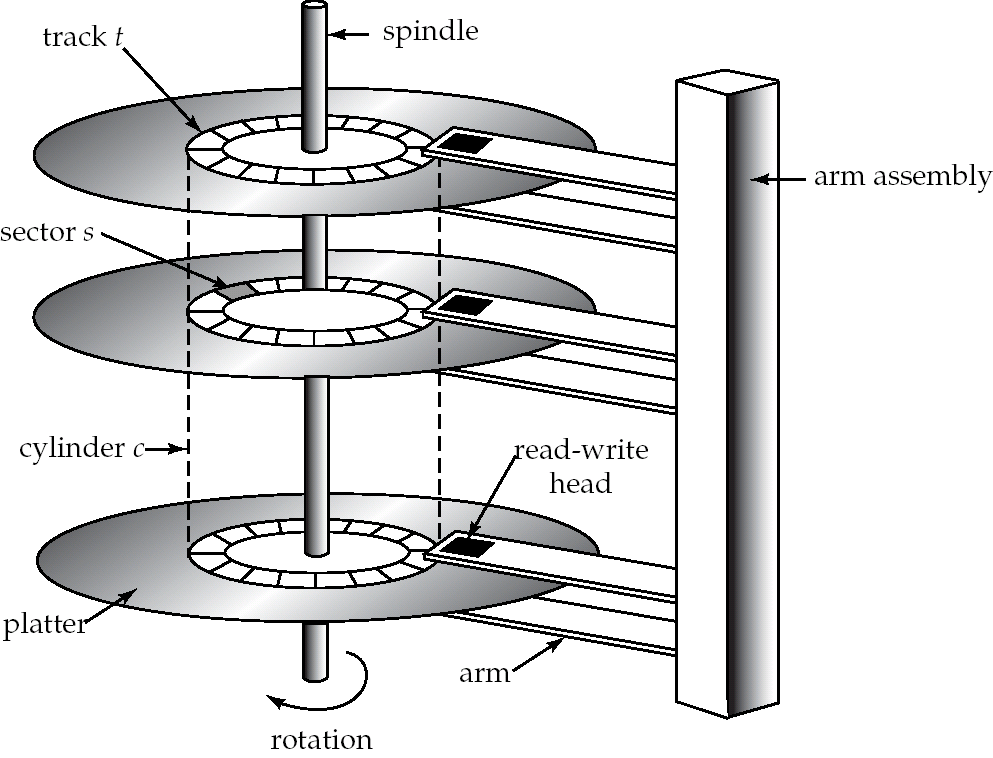
\includegraphics[scale=0.2]{img/magdisk}
\par\end{center}

\noindent \emph{Disk controller}: interfaces between system and disk
drive.
\begin{enumerate}
\item Accepts commands to read or write to sector.
\item Moves disk arm to right track and reads / writes.
\item Computes and attaches checksums to each sector to verify data is read
back correctly.
\item Ensures successful writing by reading back sector after writing.
\item Performs remapping of bad sectors.
\end{enumerate}
Measuring performance:
\begin{enumerate}
\item \emph{Access time}: time for a read or write request to be issued.

\begin{enumerate}
\item \emph{Seek time}: time to reposition arm over correct track.
\item \emph{Rotational latency}: time taken for sector to be accessed.
\end{enumerate}
\item \emph{Data transfer rate}: rate at which data can be retrieved from
or stored to disk.
\end{enumerate}
Optimisations for block access:
\begin{enumerate}
\item \emph{Block}: contiguous sequence of sectors from a single track.
Units of storage allocation / data transfer.
\item \emph{Disk arm scheduling algorithms}: order pending accesses to tracks
to minimise disk arm movements.

\begin{enumerate}
\item E.g. \emph{elevator algorithm}: move disk arm in one direction until
no more requests in that direction, then reverse.
\end{enumerate}
\item \emph{File organisation}: Organise blocks to correspond how data is
accessed.

\begin{enumerate}
\item Store related information on same blocks / cylinders.
\item Files can get \emph{fragmented} over time (by additions / scattered
free blocks). Defragment utilities often available.
\end{enumerate}
\item \emph{Non-volatile write buffers}: write blocks to non-volatile RAM
(battery backed RAM or flash memory) buffer immediately.

\begin{enumerate}
\item Controller writes to disk when no other requests or if request pending
for long time.
\item Writes can be reordered to minimise disk arm movement.
\end{enumerate}
\item \emph{Log disk}: write a sequential log of block updates. Used like
non-volatile RAM. Fast since no seeks required.
\item Reorder writes to improve performance.

\begin{enumerate}
\item \emph{Journaling file systems}: write data in safe order to NV-RAM
or log disk. Otherwise risk of corruption of file system data.
\end{enumerate}
\end{enumerate}

\paragraph{Storage Access}
\begin{enumerate}
\item Minimise block transfers by keeping as many blocks as possible in
main memory.
\item \emph{Buffer}: portion of main memory available to store copies of
disk blocks.
\item \emph{Buffer manager}: subsystem responsible for allocating buffer
space.

\begin{enumerate}
\item If block already in buffer, returns memory addr.
\item Otherwise allocates space in buffer for the block, replacing some
other (usually least recently used) block if required. Replaced block
written back to disk only if it's been modified.
\item Read block from disk to buffer and return addr of block.
\end{enumerate}
\item Buffer replacement policies can be least-recently used (LRU) or more
complex:

\begin{enumerate}
\item \emph{Pinned block}: memory block to not be written back to disk.
\item \emph{Toss-immediate}: frees space as soon as has been processed.
\item \emph{MRU}: pins current block. After final tuple processed, unpins
block, and becomes MRU.
\item \emph{Statistical}.
\end{enumerate}
\end{enumerate}

\paragraph{File Organisation}

Database is a collection of \emph{files}, which is a sequence of \emph{records}.
\begin{enumerate}
\item \emph{Fixed length records}: Assume record size fixed, only holds
one particular type, different files for different relations. Deletion
- either shift all records, or free list of deleted records with links.
\item \emph{Variable length records}: e.g. \emph{Slotted page}: header contains
number of entries, end of free space, location and size of each record.
Records can be moved around. Pointers should point to header entry.
\end{enumerate}
Sequential file organisation:
\begin{enumerate}
\item For sequential processing, ordered by a \emph{search key}.
\item \emph{Deletion}: use pointer chains.
\item \emph{Insertion}: update pointer chain - if free space insert there,
otherwise in an overflow block.
\item Need to reorganise file sometimes to maintain sequential order.
\end{enumerate}
Organisation of records in files:
\begin{enumerate}
\item Heap: record can be placed anywhere in file.
\item Sequential: store records in sequential order, based on value of search
key.
\item Hashing: hash function on some attribute specifies in which block
record is placed.
\item Multitable clustering file organisation: records of several relations
stored in same file. Related records can be stored on the same block.
\end{enumerate}
Can be \emph{row-oriented} (good for selecting all attributes) or
\emph{column-oriented} (good for selecting one attribute). Can be
sorted to optimise queries like \texttt{where att \textgreater{} val}.


\section{Indexing}
\begin{enumerate}
\item An \emph{index file} consist of records (\emph{index entries}) of
the form (\emph{search-key}, pointer).

\begin{enumerate}
\item \emph{Ordered indices}: search keys in sorted order. For a sequentially
ordered file, can use a primary index (clustering index) or secondary
index.
\item \emph{Hash indices}: distributed accross buckets using hash function.
\item \emph{Dense index files}: Index record for every search-key value.
\item \emph{Sparse}: Index records only for some search key values.

\begin{enumerate}
\item Usually requires less space and maintenance, but slower.
\item \emph{Tradeoff}: sparse index with index entry for every block in
file.
\end{enumerate}
\item \emph{Multilevel index}: treat primary index as sequential file and
create a sparse index for it. Keep outer index small enough to fit
in main memory.
\end{enumerate}
\end{enumerate}
Keeping indices up to date:
\begin{enumerate}
\item \emph{Deletion}: delete search key, or for sparse index, replace by
next search key value.
\item \emph{Insertion}: insert search key if not present, or for sparse
index, only if new block created.
\end{enumerate}
Secondary Indices:
\begin{enumerate}
\item Points to a bucket that contains pointers to all records with that
search-key value.
\item Much more expensive to scan.
\end{enumerate}

\paragraph{B\protect\textsuperscript{+} Tree Index Files}

\begin{center}
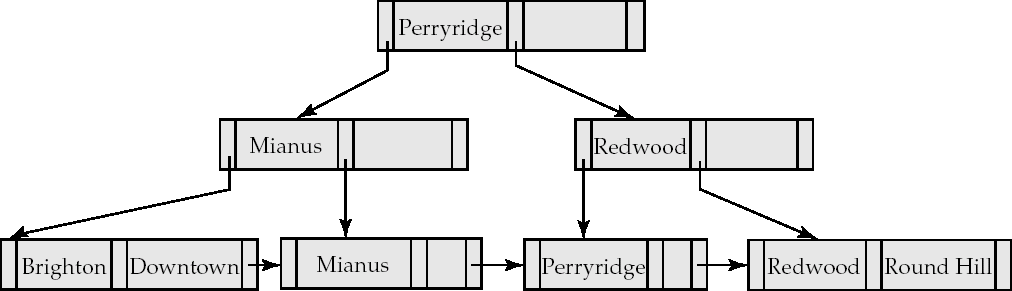
\includegraphics[scale=0.2]{img/b+tree}
\par\end{center}

\noindent Performance of indexed-sequential files degrades over time,
due to overflow blocks. B\textsuperscript{+} trees are a better solution:
\begin{enumerate}
\item All paths from root to leaf are the same length.
\item Each node that is not a root or leaf has between $\left\lceil n/2\right\rceil $
and $n$ children.
\item A leaf node has between $\left\lceil \left(n-1\right)/2\right\rceil $
and $n-1$ values.
\item \emph{Node structure}: $\left(P_{0},K_{1},P_{1},\dots,K_{n},P_{n}\right)$,
where $K$ are search key values, $P$ are pointers to children /
records / buckets of records.
\end{enumerate}
\emph{Insertion}: Insert if room on leaf node, otherwise split node
and propogate upwards.

\begin{center}
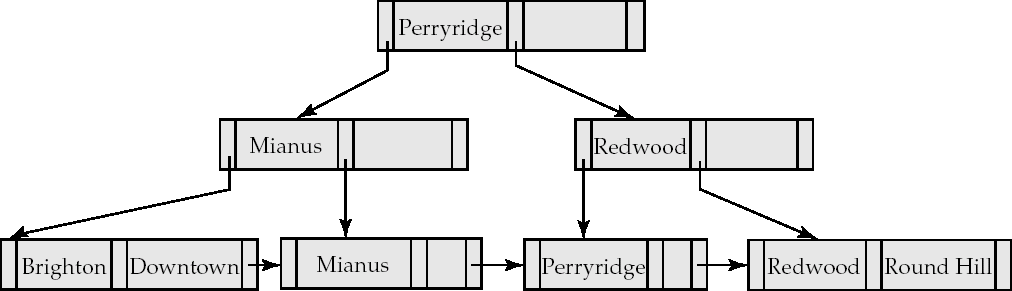
\includegraphics[scale=0.2]{img/b+tree}
\par\end{center}

\noindent \emph{Deletion}: Remove from leaf, if too few records then
merge siblings or redistribute. If node has only one pointer, then
propogate upwards.

\begin{center}
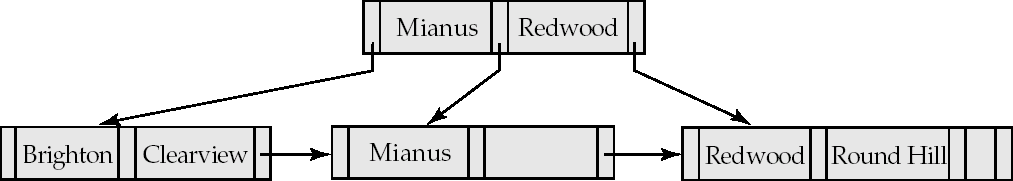
\includegraphics[scale=0.2]{img/b+delete}
\par\end{center}

\noindent Indexing of strings often uses prefix compression.


\subsection{Hashing}
\begin{enumerate}
\item \emph{Bucket} contains one or more records.
\item Obtain bucket of record using hash function.
\item Records with different search-keys may end up in the same bucket.
\end{enumerate}
Ideal hash functions are \emph{uniform} and \emph{random}.
\end{document}
